\chapter{Technology Review}
This chapter discusses the different technologies used in throughout the
project. It discusses the the advantages and disadvantages of each technology 
and why certain technologies were used over others. It also discusses hybrid applications compared to native applications, advantages, disadvantages, uses at different business structures and other topics.

\section{Overview}
This project is a Native android app built with Kotlin in Android Studio, Firebase is used for the database, statistics, verification etc.

Topics:
\begin{itemize}
    \item Kotlin/Java comparison
    \item Fire-base
    \item Picasso
    \item Android Studio/IntelliJ
    \item Native Applications
    \item Hybrid Applications
    \item Hybrid vs Native comparison 
\end{itemize}
\newpage

\section{Main Technologies}
This section will discuss the main technologies currently in use in the android application.
%----------------------------------------------------------------------------------------
% KOTLIN
%----------------------------------------------------------------------------------------
\subsection{Kotlin}
\par
\medskip
\begin{center}
    
\includegraphics[width=12cm,height=12cm,keepaspectratio]{Images/Kotlin.png}
\end{center}
Kotlin is a cross-platform, statically typed, general-purpose programming language with type inference. Kotlin is designed to inter-operate fully with Java, and the JVM version of its standard library depends on the Java Class Library, but type inference allows its syntax to be more concise. Kotlin mainly targets the JVM, but also compiles to JavaScript or native code (via LLVM). Language development costs are borne by JetBrains, while the Kotlin Foundation protects the Kotlin trademark.

Kotlin is the preferred language for Android app developers as of May 2019, since the release of Android Studio 3.0 in October 2017, Kotlin has been included as an alternative to the standard Java compiler. The Android Kotlin compiler targets Java 6 by default, and lets programmers choose between Java 8 to 14 for optimization purposes.

Kotlin originated at JetBrains, which is the company behind IntelliJ IDEA. Kotlin has been open source since 2012 and has a large team of full-time developers working on it, there is also the \hyperlink{https://github.com/JetBrains/kotlin}{Kotlin project of GitHub} which has more than 370 contributors.

\newpage

\subsubsection{Advantages}
Kotlin has many advantages, many are quite serious improvements in readability and workflow which was noticeable when creating my project

\begin{itemize}
    \item \textbf{Less code combined with greater readability} - Spend less time writing code and working to understand the code of others.
    \item \textbf{Mature language and environment} - Kotlin has developed continuously over the years not only as a language but as a whole ecosystem with very robust tooling. Its seamless integration with Android Studio, makes it actively used by companies to develop Android applications.
    \item \textbf{Kotlin support of Android Jetpack and other libraries} - \hyperlink{https://developer.android.com/kotlin/ktx}{KTX extensions} adds kotlin language features, such as coroutines, extension functions, lambdas, and named parameters, to existing Android libraries.
    \item \textbf{Interoperability with Java} - You can use Kotlin along with the Java programming language in your applications without needing to migrate all your code to Kotlin. 
    \item \textbf{Support for multi-platform development} - You can use Kotlin for developing not only Android but also iOS, back-end, and web applications by sharing the common code among the platforms.
    \item \textbf{Code safety} - Less code and better readability lead to fewer errors. The Kotlin compiler detects the remaining errors, making the code safe. 
    \item \textbf{Easy to Learn} - Kotlin is very easy to learn, especially for any Java experienced developers. 
    \item \textbf{Large community} - Kotlin a great support and many contributions from the community, which is growing all over the world. According to Google, over 60\% of the top 100 apps on the Google Play Store use Kotlin. Many startups and Fortune 500 companies have already developed Android applications using Kotlin and more and more companies are prioritizing Kotlin Native application development over other options due to the robust toolkit and optimizations that make your applications the best that they can be. 
\end{itemize}

\newpage

\subsubsection{Disadvantages}

\begin{itemize}
    \item \textbf{Shift from Java to Kotlin} - Kotlin is an amazing programming language and there is a reason why leading lead companies have started using kotlin, but at their core their two different languages. Developers won't be able to quickly shift from one to another without taking time to learn Kotlin. Therefore company's have to consider different approaches to Android app development as additional expenses are required on training a team of developers. 
    \item \textbf{Hard to find experienced developers} - There is a high demand for specialists in Kotlin as Google made it the preferred language for Android development in 2019, but there is still a very large amount of Java programmers on the market compared to Kotlin developers. This means on average the Kotlin developers may be younger meaning less senior developers available for hire. This is quite a large disadvantage, but will quickly fade away as many leading tech companies have switched which creates a ripple effect down the chain of companies.
    \item \textbf{Limited learning resources} - Although the number of Android app developers who use Kotlin instead of Java increase everyday, there is still a limited number of resources in the market compared to Java. Many College courses will teach Java over Kotlin as both are so similar, meaning most Kotlin developers come from a background in Java and learn to code in Kotlin themselves.
\end{itemize}

\newpage
\subsubsection{Kotlin Syntax}
Kotlin syntax is familiar to any programmer that is from a OOP domain and be be more or less understood from the get-go. There are differences from Java such as primary and secondary constructors, val \& var variable declarations and more.
\newline

\textbf{Below you can see the basic structure of a class in kotlin}
\begin{lstlisting}
class Foo {

    val b: String = "b"     // val means unmodifiable
    var i: Int = 0          // var means modifiable

    fun hello() {
        val str = "Hello"
        print("$str World")
    }

    fun sum(x: Int, y: Int): Int {
        return x + y
    }

    fun maxOf(a: Float, b: Float) = if (a > b) a else b

}
\end{lstlisting}

\textbf{String Interpolation} - A smarter and more readable version of Java's String.format() that is built into the language
\begin{lstlisting}
val x = 5
val y = 10
print("sum of $x and $y is ${x + y}")  // sum of 5 and 10 is 15
\end{lstlisting}

\textbf{Type Inference} - Kotlin will infer your types wherever you feel it will improve readability
\begin{lstlisting}
val a = "abc"                         // type inferred to String
val b = 4                             // type inferred to Int

val c: Double = 0.7                   // type declared explicitly
val d: List<String> = ArrayList()     // type declared explicitly
\end{lstlisting}

\textbf{Smart Casts} - The Kotlin compiler tracks logic and auto-casts types if possible, which means you do not need to use instanceof checks followed by explicit casts
\begin{lstlisting}
if (obj is String) {
    print(obj.toUpperCase())     // obj is now known to be a String
}
\end{lstlisting}

\textbf{When Expression} - The switch case is replaced with the more readable and flexible when() expression
\begin{lstlisting}
when (x) {
    1 -> print("x is 1")
    2 -> print("x is 2")
    3, 4 -> print("x is 3 or 4")
    in 5..10 -> print("x is 5, 6, 7, 8, 9, or 10")
    else -> print("x is out of range")
}

// It also works as an expression or a statement
// with or without an argument
val res: Boolean = when {
    obj == null -> false
    obj is String -> true
    else -> throw IllegalStateException()
}
\end{lstlisting}

\textbf{Setter \& Getter behavior} - You can make custom set \& get behaviors that are added to public fields, which means getter \& setters won't bloat your code
\begin{lstlisting}
class Frame {
    var width: Int = 800
    var height: Int = 600

    val pixels: Int
        get() = width * height
}
\end{lstlisting}

\textbf{Data Classes} - We frequently create classes whose main purpose is to hold data. In such a class some standard functionality and utility functions are often mechanically derivable from the data. In kotlin, this is called a data class and is marked as data. Its a Plain Old Java Object so its complete with toString(), equals(), hashCode() and copy().
\begin{lstlisting}
data class Person(val name: String,
                  var email: String,
                  var age: Int)

val john = Person("John", "john@gmail.com", 112)
}
\end{lstlisting}
%----------------------------------------------------------------------------------------
% KOTLIN VS. JAVA
%----------------------------------------------------------------------------------------
\subsection{Kotlin vs. Java in Context of Android Development}
\par
\medskip
\begin{center}
    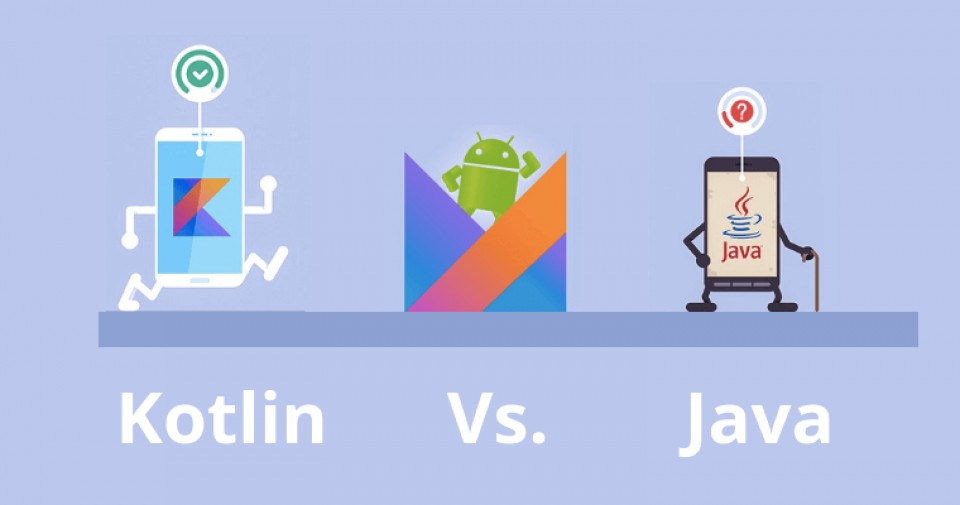
\includegraphics[width=10cm,height=10cm,keepaspectratio]{Images/KotlinvJava.jpg}
\end{center}

\subsection{Why would a Java Developer switch to Kotlin?}
Android development has always been tagged with Java Development. But Kotlin has outpaced it in performance, simplicity, maintainability, robustness, and lightweight code. Developers and users lure for feature-rich, effective and cost-efficient mobile apps that help increase the efficiency of processes, increasing competencies, meet customers’ expectations, help maintain business’ reputation and remove uncertainty. This is why Google has made Kotlin as the preferred language for Android app developers.\newline

Although Kotlin seems to work back to back with Java for front-end development, it is already being utilized in backend projects like Spring 5. It can compile to almost every platform including Android, JVM, Native and JavaScript and can extract one common code-base that will target all of them at the same time. Its scripting capabilities make it easy to handle all Gradle build scripts. Its built-in null safety support makes it win over Android that is full of old Java-style API’s. Being compatible with all Java libraries and frameworks, the JVM, Gradle integration and Maven build systems, it allows Android developers to write new modules and write them alongside existing Java code. Plus it supports modern programming concepts like higher-order functions, extension functions, delegates which help build clean API’s.
\newpage

\subsection{Why Java isn't preferred for Android Development}
\begin{itemize}
    \item \textbf{Support a subset of Java 8 Features} - Android Developers are not able to reap the full benefits of Java. To make full use of Java you must use Java 7. \cite{android_sup_java}
    \item \textbf{Issues addressed in Kotlin} - Java comes with some well-documented language issues like endless try-catch blocks, null-unsafety, NullPointerExceptions and lack of extendability that are addressed with kotlin.
    \item \textbf{Syntax of Java} - Syntax of Java is very complex and writing longer code leans to more errors, bugs and is much harder to read.
\end{itemize}

\subsection{Switch from Java to Kotlin}
\begin{itemize}
    \item \textbf{Kotlin and Java can co-exist} - Kotlin is simultaneously operable with Java. You can have both Java and Kotlin code co-exist within a single project. Both codes can compile perfectly and users are not even able to make out which part of the code is Kotlin and which part is Java.
    \item \textbf{Kotlin and Java classes can be written simultaneously} - There is no requirement to convert the entire project to Kotlin or starting a new project. Alternatively, small chunks of codes can be written in Kotlin and can be inserted as and when required, without affecting the entire code.
    \item \textbf{Kotlin is an enhancement of Java} - a java developer or an existing java application user will be easily able to comprehend what Kotlin code is doing. It looks familiar, the code is easy to read and understand.
   \item \textbf{Android Studio support for Kotlin} - Android studio has an excellent support for Kotlin. After you install Kotlin plugin, Android Studio makes it easy to configure Kotlin plugin in your project. Once this is done, the IDE will automatically understand the underlying functionality like Kotlin code compilation, and execution. Debugging, code navigation, unit testing, auto-completion and full refactoring support. Once all of this is set, converting an entire Java code into Kotlin can be accomplished in a single click.
\end{itemize}
\newpage

%----------------------------------------------------------------------------------------
% FIREBASE
%----------------------------------------------------------------------------------------
\subsection{Firebase}
\par
\medskip
\begin{center}
    
\includegraphics[width=12cm,height=12cm,keepaspectratio]{Images/firebase.png}
\end{center}

Firebase is Google's mobile and web application development platform that helps you build, improve, and grow your application. Firebase frees developers to focus on crafting excellent user experiences. You don't need to manage servers. You don't need to write APIs. Firebase is your server, your API and your database, everything is written generically so that you can modify everything to suit most needs. Firebase has a huge amount of features, real time databases, cloud storage, hosting, machine learning, authentication, statistics, analytics and more.\newline

Firebase products are setup in three different area's.
\begin{enumerate}
  \item \textbf{Build better apps}
  \item \textbf{Improve app quality}
  \item \textbf{Grow your business}
\end{enumerate}

\subsubsection{Build better apps} Firebase lets you build more powerful, secure and scalable apps, using world-class infrastructure. There are seven different products focused on building a better app. My project takes advantage of Authenication, Realtime Database and Cloud storage. Almost all of Firebase products are extremely useful and are worth mentioning as they could be implemented into the project at some point.
I will first summarize the products, and then go into further detail on the specific products i used in my project. How the code is implemented, why i used it etc.

\newpage
\subsubsection{Products for building better apps}
\begin{itemize}
    \item \textbf{Cloud Firestore} - Store and sync data between users and devices - at global scale - using a cloud-hosted, NOSQL database. Cloud Firestore gives you live synchronization and offline support along with efficient data queries. Its integration with other Firebase products enables you to build truly serverless apps.
    \item \textbf{ML Kit} - Bring powerful machine learning features to your mobile app whether you're new or experienced in ML. Get started easily by using our ready-to-use APIs for common mobile use cases, or import your own custom models which can be hosted and served to your apps by Firebase. ML Kit APIs can run on-device or in the cloud, depending on the functionality, and some give you both choices.
    \item \textbf{Cloud Functions} - Extend your app with custom backend code without needing to manage and scale your own servers. Functions can be triggered by events, which are emitted by Firebase products, Google Cloud services, or third parties, using webhook
    \item \textbf{Authentication} - Manage your users in a simple and secure way. Firebase Auth offers multiple methods to authenticate, including email and password, third-party providers like Google or Facebook, and using your existing account system directly. Build your own interface, or take advantage of our open source, fully customizable UI.
    \item \textbf{Hosting} - Simplify your web hosting with tools made specifically for modern web apps. When you upload your web assets, we automatically push them out to our global CDN and give them a free SSL certificate so your users get a secure, reliable, low-latency experience, no matter where they are.
    \item \textbf{Cloud Storage} - Store and share user-generated content like images, audio, and video with powerful, simple, and cost-effective object storage built for Google scale. The Firebase SDKs for Cloud Storage add Google security to file uploads and downloads for your Firebase apps, regardless of network quality.
    \item \textbf{Realtime Database} - Realtime Database is Firebase's original database. It's an efficient, low-latency solution for mobile apps that require synced states across clients in realtime. We recommend Cloud Firestore instead of Realtime Database for most developers starting a new project.
\end{itemize}

\newpage
\subsubsection{Improve app quality}
Firebase gives you insights into app performance and stability, so you can channel your resources effectively.
These products weren't used in the project, but are worth mentioning as they are quite valuable in a commercial development environment where app performance and crashing have a huge impact on user engagement and app performance on the Google Play Store.

\subsubsection{Products for improving app quality}
\begin{itemize}
    \item \textbf{Crashlytics} - Reduce your troubleshooting time by turning an avalanche of crashes into a manageable list of issues. Get clear, actionable insight into which issues to tackle first by seeing the user impact right in the Crashlytics dashboard. Realtime alerts will help you stay on top of stability even on the go. Crashlytics is the primary crash reporter for Firebase.
    \item \textbf{Performance Monitoring} - Diagnose app performance issues occurring on your users’ devices. Use traces to monitor the performance of specific parts of your app and see a summarized view in the Firebase console. Stay on top of your app’s start-up time and monitor HTTP requests without writing any code.
    \item \textbf{Test Lab} - Run automatic and customized tests for your app on virtual and physical devices hosted by Google. Use Firebase Test Lab throughout your development lifecycle to discover bugs and inconsistencies so that you can offer up a great experience on a wide variety of devices.
    \item \textbf{App Distribution} - Firebase App Distribution allows developers to send pre-release versions of their app to trusted testers from the console or using command line tools, as well as manage testers in one place.
\end{itemize}


\newpage
\subsubsection{Grow your business}
Firebase helps you grow to millions of users, simplifying user engagement and retention.

\subsubsection{Products for Growing your business}
\begin{itemize}
    \item \textbf{In-App Messaging} - Engage and nurture your active users with targeted and contextual messages that encourage them to complete meaningful actions within your app. You have the power to trigger messages based on user behavior and interests. You can also customize the design of in-app messages to fit your brand. In-App Messaging supports a variety of use cases and formats.
    \item \textbf{Google Analytics} - Analyze user attributions and behavior in a single dashboard to make informed decisions on your product roadmap. Gain realtime insights from reports, or export your raw event data to Google BigQuery for custom analysis.
    \item \textbf{Predictions} - Harness the power of Google’s machine learning to get insight into which segments of users are likely to churn or spend (or complete another conversion event). Use these smart predictive segments for targeting in other products like Remote Config, Cloud Messaging, and In-App Messaging.
    \item \textbf{A/B Testing} - Improve your app by running product and marketing experiments, without worrying about setting up the infrastructure to run A/B tests. Customize experiments to suit your goals. Test a variety of updates to your app, like message copy or new features. Then, only roll-out changes proven to move the needle on your key metrics.
    \item \textbf{Cloud Messaging} - Send messages and notifications to users across platforms—Android, iOS, and the web—for free. Messages can be sent to single devices, groups of devices, or specific topics or user segments. Firebase Cloud Messaging (FCM) scales to even the largest apps, delivering hundreds of billions of messages per day.
    \item \textbf{Remote Config} - Customize how your app renders for each user. Change the look and feel, roll out features gradually, run A/B tests, deliver customized content to certain users, or make other updates without deploying a new version—all from the Firebase console. Monitor the impact of your changes and make adjustments in a matter of minutes.
    \item \textbf{Dynamic Links} - Use Dynamic Links to deliver a customized user experience for iOS, Android, and the web. You can use them to power mobile web to drive native app conversions, user to user sharing, social and marketing campaigns, and more. Dynamic Links provides you with the attributions you need to better understand your mobile growth.
    
    
\end{itemize}



\subsubsection{Traditional Architecture vs. Serverless Architecture}
\begin{center}
    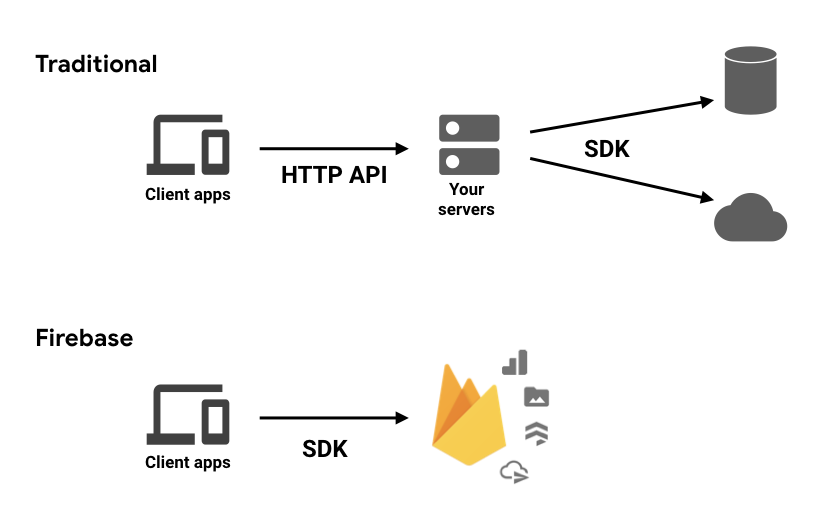
\includegraphics[width=10cm,height=10cm,keepaspectratio]{Images/firebasetradpic.png}
\end{center}

Firebase and other serverless architectures have rapidly emerged as a new technology concept in recent years. Using this Architecture, developers can create a variety of applications for various industries. Many enterprises have already started adopting serverless products, serverless architecture provides computation-light, highly-flexible, stateless applications and more. Developers are constantly on the lookout for more effective ways to maintain the software development lifecycle, doing so introduces new technologies that are accompanied with an increase in productivity. \newline
Serverless architecture was introduced to help businesses focus on application development. With serverless, businesses no longer have to worry about server infrastructure, reducing development costs and shortening the development cycle.\newline

A traditional architecture approach is frequently a large computer or cluster of computers that is accessed over the internet to provide access to information or servers. The machines are commonly located at specific area's around the world depending the size of the company. A traditional approach requires a team to manage these servers that which starts to become a problem what different scales of companies. As you get towards Enterprise sized servers they can become increasingly expensive. Not only do they cost Hundreds of Thousands to millions, you need to have space to house them, a staff of engineers to maintain them. In addition, the average life cycle of a given server is about 5 years. Which means not only do you have to potentially replace your machines, but in the interim you are constrained by the limitations of that machine.\newline
An example of these would be if a websites server does not have the capacity to handle it's increased load, the only traditional solution is to purchase more servers to handle extra volume, or replacing existing servers with a better model. Both have exceptionally high cost and come with large downsides.\newline
\newpage

Serverless Architectures aims to solve these problems. Rather than having one machine to host a job, you can now utilize servers, such as Firebase, Amazon AWS and other cloud hosted databases. All have a huge array of additional features that you opt into to spec out a server that fits your needs and removes the additional costs and headaches of a traditional server.

\begin{figure}[h!]
	\caption{Serverless Evolution}
	\label{image:myImageName}
	\centering
	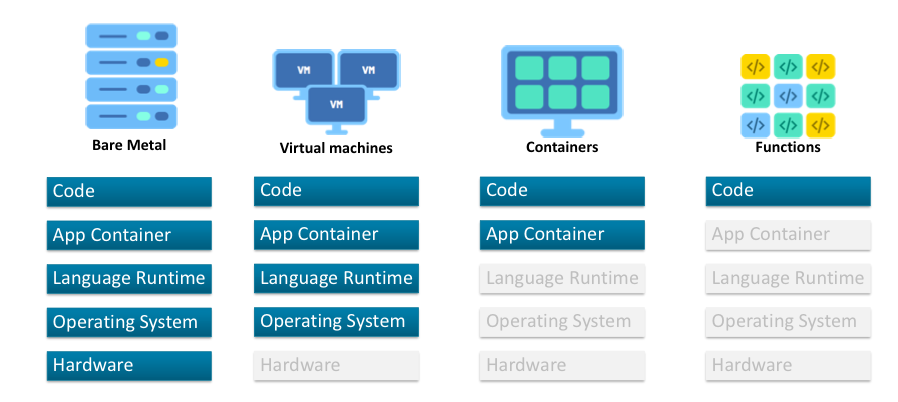
\includegraphics[width=0.8\textwidth]{Images/serverless_evolution.png}
\end{figure}




\subsubsection{Advantages of Serverless}
Advantages Serverless architectures has are the following:
\begin{enumerate}
  \item Providers scale and manages the required resources
  \item Rapid provision of resources in real-time, even for unforeseen peak loads and disproportionate growth
  \item Highly scalable and flexible architecture
  \item Users only need to pay for the resources they use
  \item High error tolerance thanks to flexible hardware infrastructure in the provider’s computer centers
\end{enumerate}

\subsubsection{Disadvantages of Serverless}
Disadvantages Serverless architectures has are the following:
\begin{enumerate}
  \item No access to virtual machines, operating system or runtime environments
  \item Implementing serverless structures is very labor-intensive
  \item Lock-in effect – for example, when changing provider, you generally have to recode all event-based functions
  \item Relatively complex monitoring and debugging process, as in-depth performance, and error analyses are generally not possible
\end{enumerate}
\newpage

As shown Firebase is an excellent option for any developer interested in creating a mobile application, finally i will go over the Pros and Cons of choosing Firebase

\subsubsection{The Pros of Firebase}
\begin{itemize}
    \item \textbf{Databases} - Depending on your budget, Google offers robust databases to use with your apps. Both realtime and Firestore databases can be scaled in terms of size, suggesting a fully secure managed solution, that still provides you easy access to your data via firebase console. Data updates and offline access makes databases usable for real time application, as well as keeping multiple databases in sync
    \item \textbf{Wide selection of products} - Firebase suggest a lot of products to make your application work. You can choose between realtime databases and firestore, store data in the cloud and build serverless applications with the integrated Cloud functions.
    \item \textbf{Free to use for small developers} - Firebase pricing\cite{firebase_pricing} is free as you start with it. This will allow you to understand whether it fits your application and understand all the peculiarities. Once you reach certain amount of database memory or need a specific product, you can choose a different plan around that product or memory you need. You can do this by using the Blaze plan calculator provided on firebase pricing website\cite{firebase_pricing}
    \item \textbf{Excellent Documentation} - The whole firebase platform is extremely well documented. Good technical documentation, API documentation, SDK references, which makes all the products easier to use and accessible for the user. The firebase products page contains all the required information concerning the integration's, available platforms, guidance's, docs, guides and lists supported technologies.
    \item \textbf{Accessible UI and ease of Integration} - Firebase requires minimal programming language knowledge, and suggests integration's via its user interface, it also is integrated into Android Studio which further increases ease of use. While eliminating the need for complex configurations, anyone can set up the application.
    \item \textbf{Google products} - Firebase comes with a Content Delivery Network (CDN) in-built with Google Cloud platform, while also having integration with all google products. A product owned by google also has the advantage of unlikely hood of the company collapsing or not supporting the product frequently.
    
\end{itemize}

\newpage
\subsubsection{The Cons of Firebase}
The cons of firebase are limited and depends on the scope of you project and the size of your company. Some of the cons are currently being fixed through new features that are currently in Beta. For example Firebase Realtime Database, which i used in this project has limitations of not being able to do complex query's and Data Modeling. Google aims to fix this with its new product Firestore. 
\begin{itemize}
    \item \textbf{Firebase Realtime Database limitations} - Realtime Database is used as the main storage for my project, which has cons. One of the mains problems with it, is the limited querying capabilities. Realtime database provides no way to filter capabilities, because the whole Database is a huge JSON file, which makes it pretty difficult to make complex queries.
    \item \textbf{Data Modeling} - Firebase Realtime Database and it data modeling as a problem where because of "Database as a single JSON file" structure,m you can't implement relations between data items.
    \item \textbf{Locked into a vendor} - This is a wide problem with BaaS solutions in general, not having the ability to migrate data to another platform can be considered a con.
     \item \textbf{Support for iOS} - While firebase is a cross-platform product, it concentrates more on Android mobile platform being that its a google product. Android Studio easily integrates all Firebase products such as Test Lab, Auth etc. While iOS devices are lacking behind on such integration's.
\end{itemize}
\newpage

%----------------------------------------------------------------------------------------
% PICASSO IMAGE HANDLING
%----------------------------------------------------------------------------------------
\subsection{Picasso}
\par
\medskip
\begin{center}
    
\includegraphics[width=10cm,height=10cm,keepaspectratio]{Images/picasso.png}
\end{center}
Picasso is a powerful image downloading and caching library, it is widely used and requires very little code to implement.
This is used because working with images in android is difficult, you need to work with network requests, caching, background threads and decoding \& encoding of image which uses a lot of memory. Picasso hides all this and adds additional features like resizing images while being memory efficient.\newline

Images add much-needed context and visual flair to Android applications. Picasso allows for hassle-free image loading in your application—often in one line of code!

\begin{lstlisting}
Picasso.get().load("http://i.imgur.com/DvpvklR.png").into(imageView);
\end{lstlisting}


Many common pitfalls of image loading on Android are handled automatically by Picasso:
\begin{itemize}
    \item Handling ImageView recycling and download cancellation in an adapter.
    \item Complex image transformations with minimal memory use.
    \item Automatic memory and disk caching.
\end{itemize}

\begin{center}
    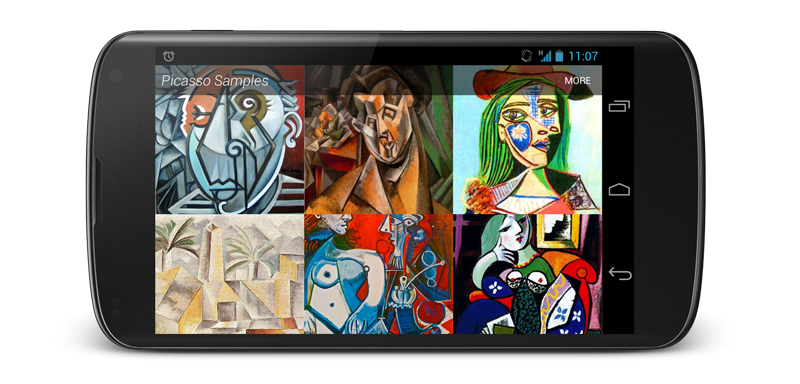
\includegraphics[width=10cm,height=10cm,keepaspectratio]{Images/picassoex1.png}
\end{center}
\newpage

\subsubsection{Features}

\textbf{ADAPTER DOWNLOADS}\newline
Adapter re-use is automatically detected and the previous download canceled.
\begin{lstlisting}
@Override public void getView(int position, View convertView, ViewGroup parent) {
  SquaredImageView view = (SquaredImageView) convertView;
  if (view == null) {
    view = new SquaredImageView(context);
  }
  String url = getItem(position);

  Picasso.get().load(url).into(view);
}
\end{lstlisting}


\textbf{IMAGE TRANSFORMATIONS}\newline

Transform images to better fit into layouts and to reduce memory size.
\begin{lstlisting}
Picasso.get()
  .load(url)
  .resize(50, 50)
  .centerCrop()
  .into(imageView)
\end{lstlisting}
\textbf{Can also specify custom transformations for more advanced effects.}
\begin{lstlisting}
public class CropSquareTransformation implements Transformation {
  @Override public Bitmap transform(Bitmap source) {
    int size = Math.min(source.getWidth(), source.getHeight());
    int x = (source.getWidth() - size) / 2;
    int y = (source.getHeight() - size) / 2;
    Bitmap result = Bitmap.createBitmap(source, x, y, size, size);
    if (result != source) {
      source.recycle();
    }
    return result;
  }

  @Override public String key() { return "square()"; }
}
\end{lstlisting}
Pass an instance of this class to the transform method.
\newpage

\textbf{PLACE HOLDERS}\newline

Picasso supports both download and error placeholders as optional features.
\begin{lstlisting}
Picasso.get()
    .load(url)
    .placeholder(R.drawable.user_placeholder)
    .error(R.drawable.user_placeholder_error)
    .into(imageView);
\end{lstlisting}
A request will be retried three times before the error placeholder is shown.\newline

\textbf{RESOURCE LOADING}\newline

Resources, assets, files, content providers are all supported as image sources.
\begin{lstlisting}
Picasso.get().load(R.drawable.landing_screen).into(imageView1);
Picasso.get().load("file:///android_asset/DvpvklR.png").into(imageView2);
Picasso.get().load(new File(...)).into(imageView3);
\end{lstlisting}

\textbf{DEBUG INDICATORS}\newline

For development you can enable the display of a colored ribbon which indicates the image source. Call setIndicatorsEnabled(true) on the Picasso instance.
\begin{center}
    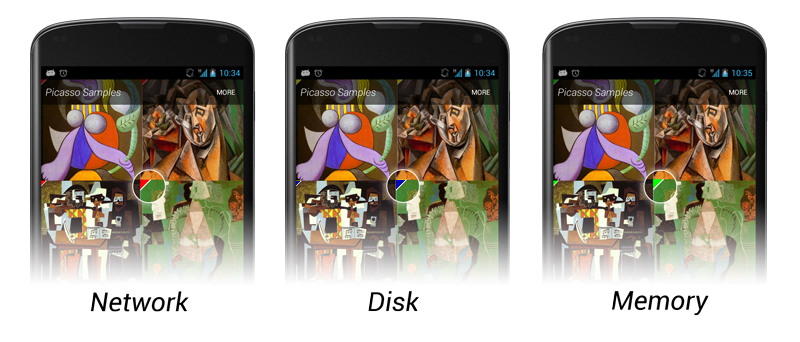
\includegraphics[width=12cm,height=12 cm,keepaspectratio]{Images/picassodebug.png}
\end{center}
\newpage

%----------------------------------------------------------------------------------------
% NATIVE APPLICATIONS
%----------------------------------------------------------------------------------------
\subsection{Native Applications}
\par
\medskip
\begin{center}
    
\includegraphics[width=12cm,height=12cm,keepaspectratio]{Images/nativeapp2.png}
\end{center}
\subsubsection{What is a Native Mobile App?}
Native Mobile applications are applications that have been written using the native development language and tools specific to that platform. For example: A native iOS application would be written in either Swift or Objective-C and compiled using Xcode, while a native android application would have been developed using Kotlin or Java and compiled using Android Studio.\newline

Since these applications are developed using the platform's default solutions, developers have full and easier access to the device's capabilities; like all the device's sensors, the user's address book, and whatever the latest and greatest new bit of technology the phone offers. Native applications tend to also be more performant since their code is closer to the 'metal'. In addition to being faster, you will also have access to all of the native user interface (UI) controls and layouts. While you will probably want to style them to fit your applications' theme, you will also want them to behave and interact like any other UI element on that platform.\newline

However, any application written in a native development language cannot be run on the opposite platform. Meaning, you have to develop separately for each platform, which leads to larger budget and team size, assuming you want to release your application on both iOS and Android. In addition, your application is only available through each platform's app stores, each having their own set of rule and restrictions. This also means that do make a new release for a new feature/fix bugs etc. you same end up having to wait a minimum of one day for it to be released.

\subsubsection{Advantages}
\begin{itemize}
    \item \textbf{Performance} - Native apps deliver the best performance of all development approaches. This is a major reason why platforms like Instagram and Airbnb \cite{react_native_ex10} \cite{react_native_ex20} moved from react native to native android development. Performance is one of the most important components of keeping a user on your application, the actions of your application need to be snappy and can't leave the user feeling like they need to wait.
    \item \textbf{Better Support} - Native apps receive complete support from app stores and the overall app marketplace. Distribution in app stores helps with discover-ability. Overtime Google has made Native development a more favoured development standard, along with the pressure of consumers waiting a extremely high standard from mobile applications. Having better support a company such as Apple or Google is a strong advantage over hybrid development.
    \item \textbf{Better Overall} - Native apps are interactive, intuitive, and run more smoothly in terms of user input and output. As mentioned native apps are just smoother for large applications.
    \item \textbf{Native Integration Features} - Native development allows developers to access the full feature set of the selected operating system. Not only do you have the full feature set from the selected operating system, you also have a the full feature set of tools like Android Studio.
    \item \textbf{Flow of app} - The user experience of native apps is far superior to web apps or hybrid apps. To the user, the flow is more natural because of each mobile operating system’s specific UI guidelines and standards.
    \item \textbf{Goggle App Store Quality} - A native app must be approved by its respective operating system which assures quality, security, and device compatibility. While all Apps on the Google App Store aren't all at the highest standard, Google has an aggressive stance on the expected quality of applications and will quickly remove a developers access to the store if they are seen to be having a negative on the store as a whole.
\end{itemize}
\subsubsection{Disadvantages}
\begin{itemize}
    \item \textbf{Higher Difficulty} - Native apps use difficult programming languages which require experienced developers.
    \item \textbf{Higher Cost} - Expenses are more costly upfront for native apps compared to web or hybrid apps.
    \item \textbf{Not the best option for Simple apps} - Native apps are not the best option for simple applications.
    \item \textbf{Hiring Experienced Developers} - Hiring experienced native developers can be more difficult and costly compared to a hybrid developer.
\end{itemize}
\newpage
\subsection{Hybrid Applications}
\par
\medskip
\begin{center}
    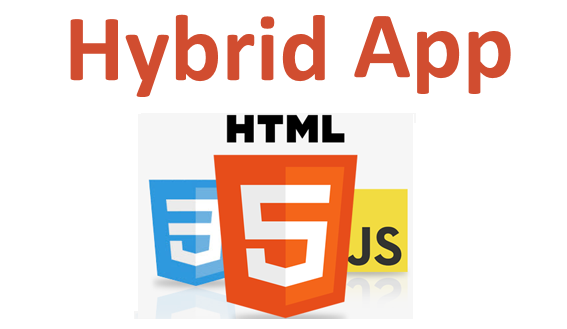
\includegraphics[width=10cm,height=10cm,keepaspectratio]{Images/hybridapp.png}
\end{center}

\subsubsection{What is a Hybrid App?}
Hybrid apps are a blend, hence the name hybrid, of both native and web solutions. Where the core of the application is written using web technologies.\newline

The core of an hybrid application is written using web technologies (HTML, CSS and JavaScript), which are then encapsulated within a native application. Through the use of plugins, these applications can have full access to the mobile device’s features.\cite{ionic_hybid_app}\newline

The heart of a hybrid-mobile application is still just an application that is written with HTML, CSS, and JavaScript. However, instead of the app being shown within the user’s browser, it is run from within a native application and its own embedded browser, which is essentially invisible to the user. For example, an iOS application would use the WKWebView to display our application, while on Android it would use the WebView element to do the same function.\cite{ionic_hybid_app}\newline

This code is then embedded into a native application wrapper using a solution like \hyperlink{https://cordova.apache.org/docs/en/latest/guide/overview/}{Apache Cordova} and creates a native shell application that is just the platform’s webview component in which it will load your web application. This gives you the ability to create and publish true native applications that can be submitted to each of the platform’s app stores for sale.

\begin{figure}[h!]
	\caption{Architecture of a Hybrid App (Cordova) \cite{cordova_hybid_app}}
	\label{image:myImageName}
	\centering
	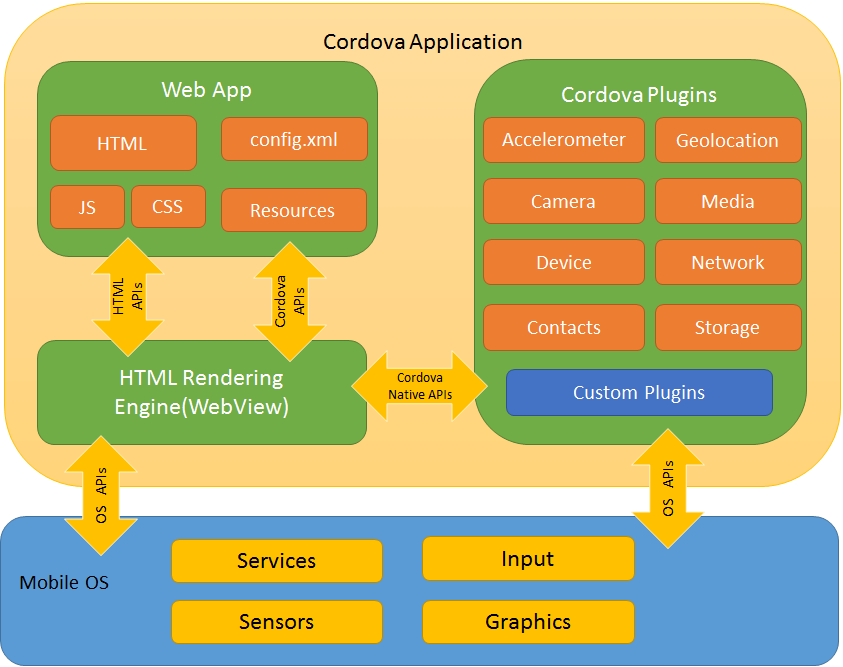
\includegraphics[width=1\textwidth]{Images/cordovaapparchitecture.png}
\end{figure}	

\newpage
\subsubsection{When to use Hybrid Applications}
Hybrid mobile applications have their place in situations where fast development is the main priority or when the high cost of targeting each separate platform with an individual native application would prohibit the creation of the application. Large companies who are in an extremely competitive app market are not going to sacrifice performance and control with hybrid development. However smaller developers have the option of taking advantage of the gap between native and hybrid development in terms of the most cost effective options and when it comes to cost hybrid development is very cost effective for a lot of companies.


\subsubsection{Advantages}
\begin{itemize}
    \item \textbf{Unified Development} - By far the single biggest benefit that hybrid mobile apps can offer is the unified development. Companies can save a substantial amount of money that would otherwise have to be spent on developing and maintaining separate code bases for different mobile platforms. They can develop just a single version and let their hybrid framework of choice do the heavy lifting and ensure that everything will work flawlessly.
    This, of course, directly leads to lower cost of development and, potentially, greater revenue. Many small businesses wouldn’t be able to afford to target all major mobile platforms, if there wasn’t the option to do so with a hybrid framework.
    \item \textbf{Fast Deployment} - The Minimum Viable Product (MVP) approach necessitates the fast deployment of functional solutions in order to be the first to penetrate the market and gain a substantial competitive advantage. Those who need to have their app in the App Store as fast as possible should seriously consider using hybrid applications.\cite{mvp_paper}
    \item \textbf{Scaling} - Hybrid applications are limited only by the underlying framework. Companies who partner with a good provider can instantly target all major platforms without any additional effort at all. It the platform is popular enough, it can be expected that it will quickly add support for any new mobile operating systems and their respective incremental updates.
    \item \textbf{Return on Investment} - Hybrid applications built with software such as Ionic have, 1. 60-80\% time savings on average building with hybrid versus native. 2. Less hiring costs. 3. Project is more feasible with lower costs. \cite{ionic_hybrid_roi}
\end{itemize}

\subsubsection{Disadvantages}
\begin{itemize}
    \item \textbf{App Performance} - Hybrid apps add an extra layer between the source code and the target mobile platform: the particular hybrid mobile framework, such as Ionic, Cordova, Xamarin, React Native, and many others. The unsurprising result is a possible loss of performance. It really varies from application to application just how noticeable the difference can be, but the fact that Facebook migrated their mobile application from HTML5 to native shows that there really can be a significant difference, at least for large-scale applications. Mark Zuckerberg even went on to say that “The biggest mistake we've made as a company is betting on HTML5 over native.”
    \item \textbf{Debugging} - That extra layer also makes debugging a potential nightmare. Developers have to rely on the framework itself to play nicely with the targeted operating system and not introduce any new bugs. Since developers are not likely to have a deep knowledge of the targeted platform, figuring out the exact cause of an issue can be a lengthy affair.
    \item \textbf{Lack native features} - Hybrid apps lack the integration with native operating systems that limit to app at certain points, once your app reaches a certain point of complexity Hybrid apps start to struggle.
\end{itemize}
%
%\subsection{Hybrid vs Native Applications}
%\par
%\medskip
%\begin{center}
%    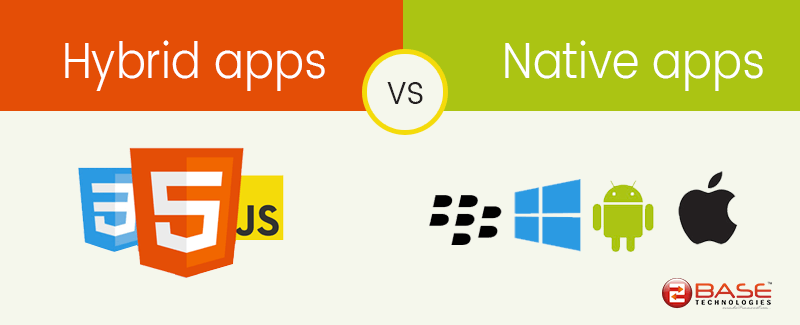
\includegraphics[width=12cm,height=12cm,keepaspectratio]{Images/hybridvnative.png}
%\end{center}%
%
%blah..%
%
%
%\subsubsection{Advantages}
%\begin{itemize}
%    \item \textbf{Shift from Java to Kotlin} - Kotlin
%%    \item \textbf{Hard to find experienced developers} - asdas
%    \item \textbf{Limited learning resources} - Although
%\end{itemize}
%\subsubsection{Disadvantages}
%\begin{itemize}
%    \item \textbf{Shift from Java to Kotlin} - Kotlin
%    \item \textbf{Hard to find experienced developers} - asdas
%    \item \textbf{Limited learning resources} - Although
%\end{itemize}
%